% LaTeX Template for short student reports.
% Citations should be in bibtex format and go in references.bib
\documentclass[a4paper, 11pt]{article}
\usepackage[top=3cm, bottom=3cm, left = 2cm, right = 2cm]{geometry} 
\geometry{a4paper} 
\usepackage[utf8]{inputenc}
\usepackage{textcomp}
\usepackage{graphicx} 
\usepackage{mathtools}
\usepackage{diffcoeff}
\usepackage{amsmath,amssymb}  
\usepackage{bm}  
\usepackage[pdftex,bookmarks,colorlinks,breaklinks]{hyperref}  
%\hypersetup{linkcolor=black,citecolor=black,filecolor=black,urlcolor=black} % black links, for printed output
\usepackage{memhfixc} 
\usepackage{pdfsync}  
\usepackage{fancyhdr}
\usepackage{movie15}
\pagestyle{fancy}

\title{PCA Report}
\author{Donal Loitam}
%\date{}

\begin{document}
\maketitle
\tableofcontents

\section{Introduction}
\begin{itemize}
    \item Principal Component Analysis, or PCA, is a dimensionality-reduction method that is often used to reduce the dimensionality of large data sets
    \item It transforms a large set of variables into a smaller one(combinations of the older variables) that still contains most of the information in the large set.
    \item \textbf{Accuracy-Simplicity Trade off: }Reducing the number of variables of a data set naturally comes at the expense of accuracy. As an added benefit, each of the “new” variables after PCA are all independent of one another
    \item Smaller data sets are easier to explore and visualize and make analyzing data much easier and faster
\end{itemize}


\section{Key Points of the Algorithm}
\begin{itemize}
    \item STANDARDIZATION :
    \begin{itemize}
        \item The aim of this step is to standardize the range of the continuous initial variables so that each one of them contributes equally to the analysis.
        \item It is critical to perform standardization prior to PCA  because the latter is quite sensitive regarding the variances of the initial variables.
        \item Ex. A variable that ranges between 0 and 100 will dominate over a variable that ranges between 0 and 1
        \begin{align}
            z = \frac{x-\mu}{\sigma}
        \end{align}
    \end{itemize} 
    \pagebreak
    \item COVARIANCE MATRIX COMPUTATION :
    \begin{itemize}
        \item We compute this matrix to idemtify if there is any significant correlation between any 2 variables because if it is the case, then we can drop one of them as it would be redundant
        \item Example of a covariance matrix having three variables $x,y,z$\\
        \begin{align}
            \begin{bmatrix}
                Cov(x,x) & Cov(x,y) & Cov(x,z)\\
                Cov(y,x) & Cov(y,y) & Cov(y,z) \\
                Cov(z,x) & Cov(z,y) & Cov(z,z)
                \end{bmatrix}  
        \end{align} 
    \end{itemize}
    \item  COMPUTE THE EIGENVECTORS AND EIGENVALUES OF THE COVARIANCE MATRIX TO IDENTIFY THE PRINCIPAL COMPONENTS:    :
    \begin{itemize}
        \item Principal components are new variables that are constructed as linear combinations or mixtures of the initial variables. 
        \item These combinations are done in such a way that the new variables (i.e., principal components) are uncorrelated/perpendicular.
        \item Geometrically, principal components represent the directions of the data that explain a \textbf{maximum variance}, or, the lines that capture most information of the data.
        \item Larger the variance carried by a line, the larger the dispersion of the data points along it, and the larger the dispersion along a line, the more the information it has
        \item PCA tries to put maximum possible information in the first component, then in the second and so on, until having something like shown in the \textbf{scree plot} below.
\begin{figure}[h!]
    \centering
    \includegraphics[width=0.7\linewidth]{scree2.png}
    \caption{Scree plot for 4 dimensions}
    \label{fig:fig1}
  \end{figure}
  \item \textbf{How PCA Constructs the Principal Components : }Let’s assume that the scatter plot of our data set is as shown below, 
  can we guess the first principal component ? Yes, it’s approximately the line 
  that matches the purple marks because it goes through the \textbf{origin(mean of all the datapoints)} and it’s the line in which the projection of the points (red dots) is the most spread out. 
  Or mathematically speaking, it’s the line that \textbf{maximizes the variance} (the average of the squared distances from the projected points (red dots) to the \textbf{origin}).
  \begin{figure}[h!]
    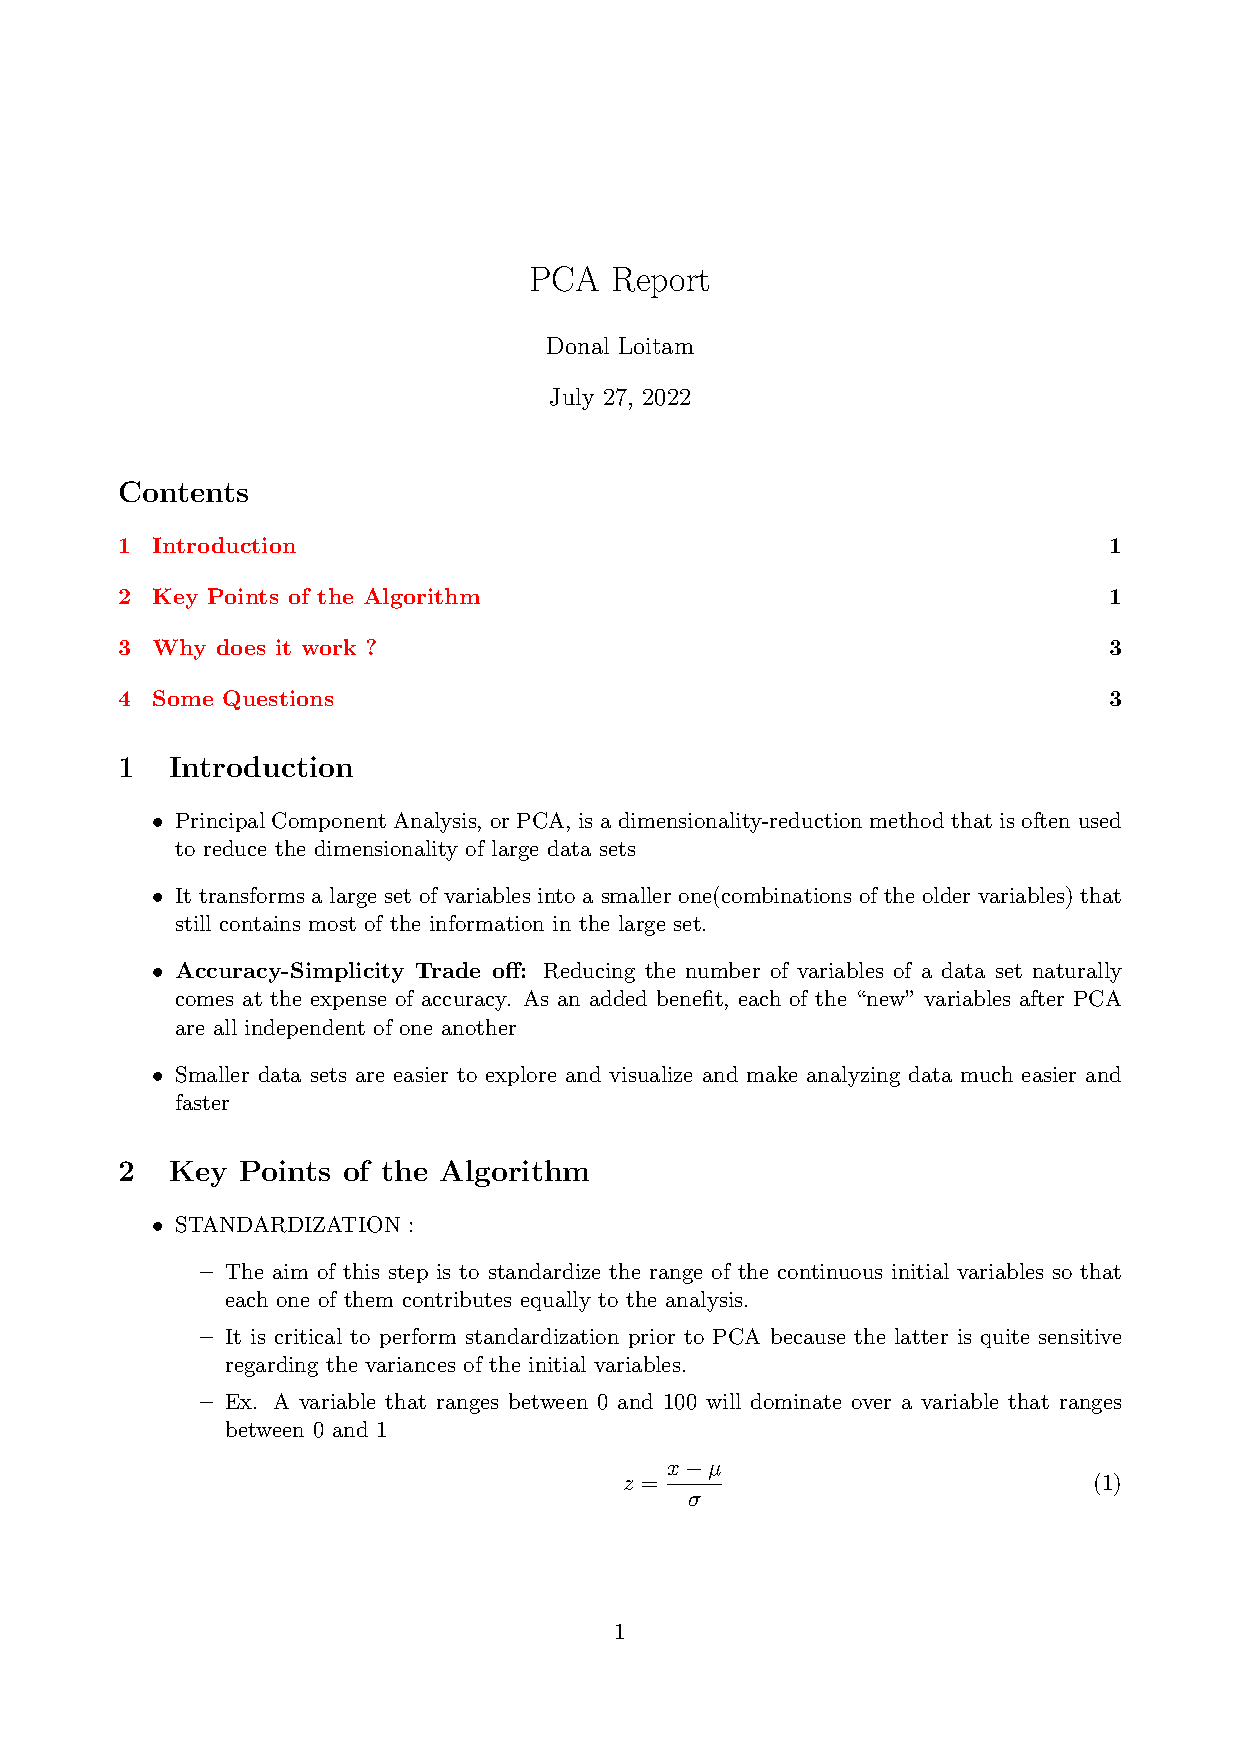
\includegraphics[width=0.7\linewidth]{pca.png}
    \caption{Finding the PCA1}
    \label{fig:fig2}
  \end{figure}
  The second principal component is calculated in the same way, with the condition that it is uncorrelated with (i.e., perpendicular to) the first principal component and that it accounts for the next highest variance.
    \end{itemize}  
\end{itemize}


\section{Why does it work ?} 
\begin{itemize}
    \item First,The eigenvectors of the Covariance matrix are actually the directions of the axes where there is the most variance(most information)
    \item Second, eigenvalues are simply the coefficients attached to eigenvectors, which give the amount of variance carried in each Principal Component.
     \item Finally, we make an assumption that more variability in a particular direction correlates with explaining the behavior of the dependent variable.
     Lots of variability usually indicates signal, whereas little variability usually indicates noise. Thus, the more variability there is in a particular direction is,
      theoretically, indicative of something important we want to detect
\end{itemize}


% \section{Unique Features}

% We did some experiments \ldots

% \pagebreak

\section{Some Questions}
1. Explain the Curse of Dimensionality?\\
\textbf{Ans.}  \begin{itemize}
    \item  As the number of features increase, the number of samples increases, hence, the model becomes more complex
    \item The more the number of features, the more the chances of overfitting. 
\end{itemize}
2. What are the pros and cons of Dimensionality Reduction ? \\
\textbf{Ans. Some advantages for Dimensionality Reduction :-} 
\begin{itemize}
\item BETTER VISUALISATION : Dimensionality Reduction helps us visualize the data on 2D plots or 3D plots.
 \item REDUCED SPACE AND TIME COMPLEXITY : Fewer dimensions mean less computing. Less data means that algorithms train faster.
\end{itemize}
\pagebreak
\textbf{While some drawbacks are :-}
\begin{itemize}
    \item LESS INTERPRETABLE FEATURE : Transformed features are often hard to interpret
     \item Some information is lost, possibly degrading the performance of subsequent training algorithms.
    \end{itemize}
3. Is rotation necessary in PCA?\\ 
\textbf{Ans :} Yes, rotation (orthogonal) is necessary to account the maximum variance of the training set. 
If we don’t rotate the components, the effect of PCA will diminish and we’ll have to select more number of components to explain variance in the training set.\\
4.  Assumptions taken while applyng PCA ?  \\
\textbf{Ans.}
 \begin{itemize}
    \item There needs to be a \textbf{linear relationship} between all variables. The reason for this assumption is that a PCA is based on Pearson correlation coefficients.
    \item For getting reliable results by using the PCA algorithm, we require a large enough sample size i.e, we
    should have sampling adequacy.
    \item  We need to have adequate correlations between the
    variables to be reduced to a smaller number of components.
\end{itemize}
5. How can you evaluate the performance of a dimensionality reduction algorithm on your dataset?
\\ \textbf{Ans. } \\
Intuitively, a dimensionality reduction algorithm performs well if it eliminates a 
lot of dimensions from the dataset without losing too much information \\ Alternatively, if you are using dimensionality reduction as a preprocessing step before another Machine Learning algorithm (e.g., a Random Forest classifier), then you can simply measure the performance of that second algorithm; if dimensionality reduction did not lose too much information, then the algorithm should perform just as well as when using the original dataset.

\bibliographystyle{abbrv}
% \bibliography{references}  % need to put bibtex references in references.bib 
\end{document}
